% Options for packages loaded elsewhere
\PassOptionsToPackage{unicode}{hyperref}
\PassOptionsToPackage{hyphens}{url}
%
\documentclass[
]{article}
\usepackage{amsmath,amssymb}
\usepackage{lmodern}
\usepackage{iftex}
\ifPDFTeX
  \usepackage[T1]{fontenc}
  \usepackage[utf8]{inputenc}
  \usepackage{textcomp} % provide euro and other symbols
\else % if luatex or xetex
  \usepackage{unicode-math}
  \defaultfontfeatures{Scale=MatchLowercase}
  \defaultfontfeatures[\rmfamily]{Ligatures=TeX,Scale=1}
\fi
% Use upquote if available, for straight quotes in verbatim environments
\IfFileExists{upquote.sty}{\usepackage{upquote}}{}
\IfFileExists{microtype.sty}{% use microtype if available
  \usepackage[]{microtype}
  \UseMicrotypeSet[protrusion]{basicmath} % disable protrusion for tt fonts
}{}
\makeatletter
\@ifundefined{KOMAClassName}{% if non-KOMA class
  \IfFileExists{parskip.sty}{%
    \usepackage{parskip}
  }{% else
    \setlength{\parindent}{0pt}
    \setlength{\parskip}{6pt plus 2pt minus 1pt}}
}{% if KOMA class
  \KOMAoptions{parskip=half}}
\makeatother
\usepackage{xcolor}
\usepackage[margin=1in]{geometry}
\usepackage{color}
\usepackage{fancyvrb}
\newcommand{\VerbBar}{|}
\newcommand{\VERB}{\Verb[commandchars=\\\{\}]}
\DefineVerbatimEnvironment{Highlighting}{Verbatim}{commandchars=\\\{\}}
% Add ',fontsize=\small' for more characters per line
\usepackage{framed}
\definecolor{shadecolor}{RGB}{248,248,248}
\newenvironment{Shaded}{\begin{snugshade}}{\end{snugshade}}
\newcommand{\AlertTok}[1]{\textcolor[rgb]{0.94,0.16,0.16}{#1}}
\newcommand{\AnnotationTok}[1]{\textcolor[rgb]{0.56,0.35,0.01}{\textbf{\textit{#1}}}}
\newcommand{\AttributeTok}[1]{\textcolor[rgb]{0.77,0.63,0.00}{#1}}
\newcommand{\BaseNTok}[1]{\textcolor[rgb]{0.00,0.00,0.81}{#1}}
\newcommand{\BuiltInTok}[1]{#1}
\newcommand{\CharTok}[1]{\textcolor[rgb]{0.31,0.60,0.02}{#1}}
\newcommand{\CommentTok}[1]{\textcolor[rgb]{0.56,0.35,0.01}{\textit{#1}}}
\newcommand{\CommentVarTok}[1]{\textcolor[rgb]{0.56,0.35,0.01}{\textbf{\textit{#1}}}}
\newcommand{\ConstantTok}[1]{\textcolor[rgb]{0.00,0.00,0.00}{#1}}
\newcommand{\ControlFlowTok}[1]{\textcolor[rgb]{0.13,0.29,0.53}{\textbf{#1}}}
\newcommand{\DataTypeTok}[1]{\textcolor[rgb]{0.13,0.29,0.53}{#1}}
\newcommand{\DecValTok}[1]{\textcolor[rgb]{0.00,0.00,0.81}{#1}}
\newcommand{\DocumentationTok}[1]{\textcolor[rgb]{0.56,0.35,0.01}{\textbf{\textit{#1}}}}
\newcommand{\ErrorTok}[1]{\textcolor[rgb]{0.64,0.00,0.00}{\textbf{#1}}}
\newcommand{\ExtensionTok}[1]{#1}
\newcommand{\FloatTok}[1]{\textcolor[rgb]{0.00,0.00,0.81}{#1}}
\newcommand{\FunctionTok}[1]{\textcolor[rgb]{0.00,0.00,0.00}{#1}}
\newcommand{\ImportTok}[1]{#1}
\newcommand{\InformationTok}[1]{\textcolor[rgb]{0.56,0.35,0.01}{\textbf{\textit{#1}}}}
\newcommand{\KeywordTok}[1]{\textcolor[rgb]{0.13,0.29,0.53}{\textbf{#1}}}
\newcommand{\NormalTok}[1]{#1}
\newcommand{\OperatorTok}[1]{\textcolor[rgb]{0.81,0.36,0.00}{\textbf{#1}}}
\newcommand{\OtherTok}[1]{\textcolor[rgb]{0.56,0.35,0.01}{#1}}
\newcommand{\PreprocessorTok}[1]{\textcolor[rgb]{0.56,0.35,0.01}{\textit{#1}}}
\newcommand{\RegionMarkerTok}[1]{#1}
\newcommand{\SpecialCharTok}[1]{\textcolor[rgb]{0.00,0.00,0.00}{#1}}
\newcommand{\SpecialStringTok}[1]{\textcolor[rgb]{0.31,0.60,0.02}{#1}}
\newcommand{\StringTok}[1]{\textcolor[rgb]{0.31,0.60,0.02}{#1}}
\newcommand{\VariableTok}[1]{\textcolor[rgb]{0.00,0.00,0.00}{#1}}
\newcommand{\VerbatimStringTok}[1]{\textcolor[rgb]{0.31,0.60,0.02}{#1}}
\newcommand{\WarningTok}[1]{\textcolor[rgb]{0.56,0.35,0.01}{\textbf{\textit{#1}}}}
\usepackage{graphicx}
\makeatletter
\def\maxwidth{\ifdim\Gin@nat@width>\linewidth\linewidth\else\Gin@nat@width\fi}
\def\maxheight{\ifdim\Gin@nat@height>\textheight\textheight\else\Gin@nat@height\fi}
\makeatother
% Scale images if necessary, so that they will not overflow the page
% margins by default, and it is still possible to overwrite the defaults
% using explicit options in \includegraphics[width, height, ...]{}
\setkeys{Gin}{width=\maxwidth,height=\maxheight,keepaspectratio}
% Set default figure placement to htbp
\makeatletter
\def\fps@figure{htbp}
\makeatother
\setlength{\emergencystretch}{3em} % prevent overfull lines
\providecommand{\tightlist}{%
  \setlength{\itemsep}{0pt}\setlength{\parskip}{0pt}}
\setcounter{secnumdepth}{-\maxdimen} % remove section numbering
\usepackage{pafpages}
\ifLuaTeX
  \usepackage{selnolig}  % disable illegal ligatures
\fi
\IfFileExists{bookmark.sty}{\usepackage{bookmark}}{\usepackage{hyperref}}
\IfFileExists{xurl.sty}{\usepackage{xurl}}{} % add URL line breaks if available
\urlstyle{same} % disable monospaced font for URLs
\hypersetup{
  pdftitle={Course2 R Programming - Assignment 3},
  pdfauthor={Haoyi Wei},
  hidelinks,
  pdfcreator={LaTeX via pandoc}}

\title{Course2 R Programming - Assignment 3}
\author{Haoyi Wei}
\date{2022-12-21}

\begin{document}
\maketitle

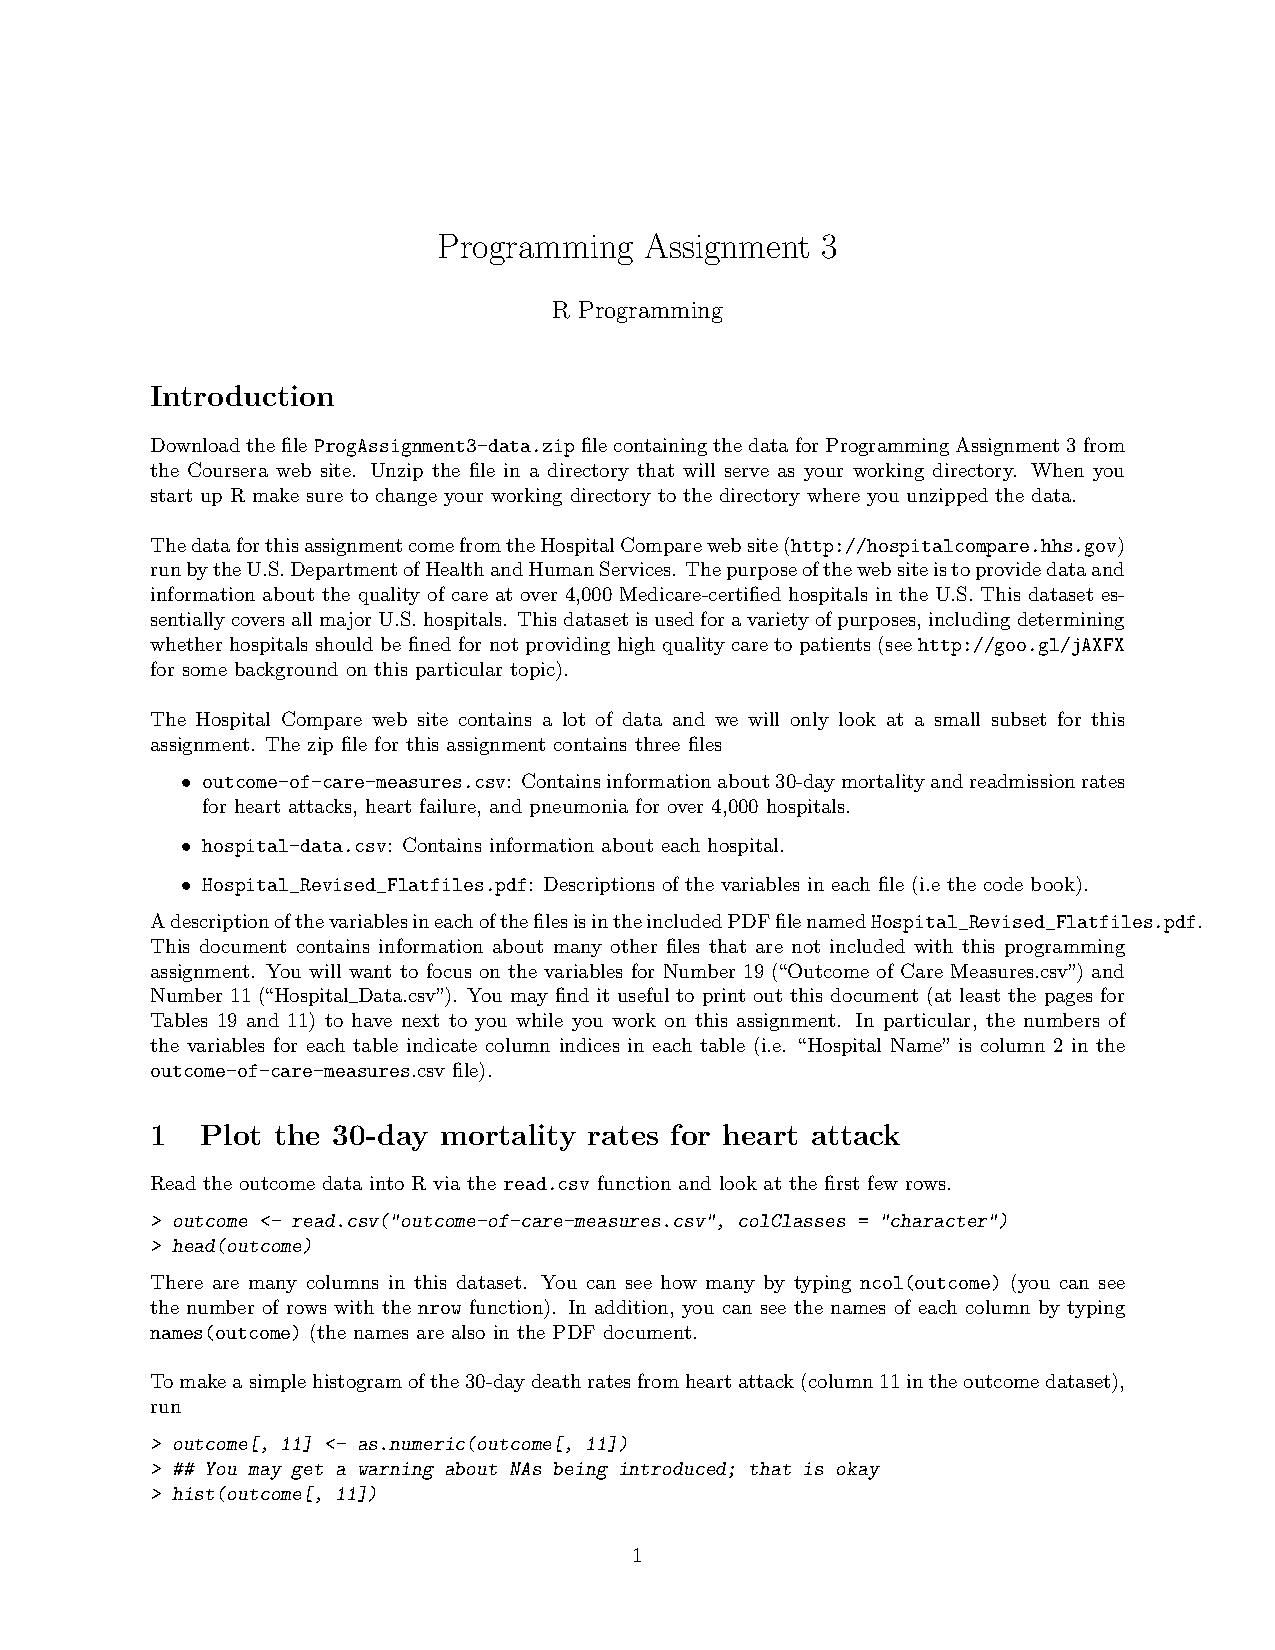
\includepdf[pages=-]{DS2-HW3-Instruction.pdf}

Programming Assignment 3

The data for this assignment come from the Hospital Compare web site
(\url{http://hospitalcompare.hhs.gov}) run by the U.S. Department of
Health and Human Services. The purpose of the web site is to provide
data and information about the quality of care at over 4,000
Medicare-certi ed hospitals in the U.S. This dataset essentially covers
all major U.S. hospitals. This dataset is used for a variety of
purposes, including determining whether hospitals should be fined for
not providing high quality care to patients.

\begin{Shaded}
\begin{Highlighting}[]
\CommentTok{\# set the working directory}
\FunctionTok{setwd}\NormalTok{(}\StringTok{"\textasciitilde{}/Documents/GitHub/Coursera\_Data\_Science\_Certificate/2\_R Programming/Code"}\NormalTok{)}
\CommentTok{\# packages}
\FunctionTok{library}\NormalTok{(dplyr)}
\end{Highlighting}
\end{Shaded}

\hypertarget{plot-the-30-day-mortality-rates-for-heart-attack}{%
\section{1 Plot the 30-day mortality rates for heart
attack}\label{plot-the-30-day-mortality-rates-for-heart-attack}}

\begin{Shaded}
\begin{Highlighting}[]
\CommentTok{\# Read the outome data into R via the read.csv function.}
\NormalTok{outcome }\OtherTok{\textless{}{-}}\FunctionTok{read.csv}\NormalTok{(}\StringTok{"./hospital/outcome{-}of{-}care{-}measures.csv"}\NormalTok{)}
\end{Highlighting}
\end{Shaded}

\begin{Shaded}
\begin{Highlighting}[]
\CommentTok{\# look at the first few rows}
\FunctionTok{head}\NormalTok{(outcome)}
\end{Highlighting}
\end{Shaded}

\begin{Shaded}
\begin{Highlighting}[]
\CommentTok{\# Check the number of column or row}
\FunctionTok{ncol}\NormalTok{(outcome)}
\end{Highlighting}
\end{Shaded}

\begin{verbatim}
## [1] 46
\end{verbatim}

\begin{Shaded}
\begin{Highlighting}[]
\FunctionTok{nrow}\NormalTok{(outcome)}
\end{Highlighting}
\end{Shaded}

\begin{verbatim}
## [1] 4706
\end{verbatim}

\begin{Shaded}
\begin{Highlighting}[]
\CommentTok{\# names of each column}
\FunctionTok{names}\NormalTok{(outcome)}
\end{Highlighting}
\end{Shaded}

\begin{Shaded}
\begin{Highlighting}[]
\CommentTok{\# To make a simple histogram of the 30{-}day death rates from heart attack (column 11 in the outcome dataset), run}

\NormalTok{outcome[, }\DecValTok{11}\NormalTok{] }\OtherTok{\textless{}{-}} \FunctionTok{as.numeric}\NormalTok{(outcome[, }\DecValTok{11}\NormalTok{])}
\end{Highlighting}
\end{Shaded}

\begin{verbatim}
## Warning: NAs introduced by coercion
\end{verbatim}

\begin{Shaded}
\begin{Highlighting}[]
\DocumentationTok{\#\# You may get a warning about NAs being introduced; that is okay}

\FunctionTok{hist}\NormalTok{(outcome[, }\DecValTok{11}\NormalTok{])}
\end{Highlighting}
\end{Shaded}

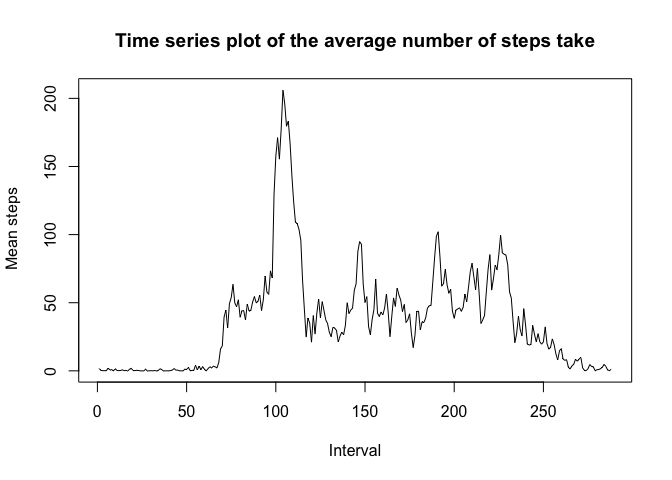
\includegraphics{DS2-HW3-html_files/figure-latex/unnamed-chunk-6-1.pdf}

\hypertarget{finding-the-best-hospital-in-a-state}{%
\section{2 Finding the best hospital in a
state}\label{finding-the-best-hospital-in-a-state}}

Write a function called best that take two arguments: the 2-character
abbreviated name of a state and an outcome name. The function reads the
outcome-of-care-measures.csv and returns a character vector with the
name of the hospital that has the best (i.e.~lowest) 30-day mortality
for the specied outcome in that state. The hospital name is the name
provided in the Hospital.Name variable. The outcomes can be one of heart
attack'', heart failure'', or pneumonia''. Hospitals that do not have
data on a particular outcome should be excluded from the set of
hospitals when deciding the rankings.

Handling ties. If there is a tie for the best hospital for a given
outcome, then the hospital names should be sorted in alphabetical order
and the  rst hospital in that set should be chosen (i.e.~if hospitals
\b", \c",and \f" are tied for best, then hospital \b" should be
returned).

The function should check the validity of its arguments. If an invalid
state value is passed to best, the function should throw an error via
the stop function with the exact message \invalid state''. If an invalid
outcome value is passed to best, the function should throw an error via
the stop function with the exact message \invalid outcome''.

\begin{Shaded}
\begin{Highlighting}[]
\NormalTok{best }\OtherTok{\textless{}{-}} \ControlFlowTok{function}\NormalTok{(st, out) \{}
  \DocumentationTok{\#\# Read outcome data}
        \DocumentationTok{\#\# clean the dataset to restricted to interested variables and convert character to numeric.}
\NormalTok{          outcome1 }\OtherTok{\textless{}{-}}\NormalTok{ outcome }\SpecialCharTok{\%\textgreater{}\%}
            \FunctionTok{select}\NormalTok{(Provider.Number,Hospital.Name,State, }\FunctionTok{starts\_with}\NormalTok{(}\StringTok{"Hospital.30.Day.Death..Mortality..Rates.from."}\NormalTok{)) }\SpecialCharTok{\%\textgreater{}\%}
            \FunctionTok{mutate}\NormalTok{(}\FunctionTok{across}\NormalTok{(}\FunctionTok{starts\_with}\NormalTok{(}\StringTok{"Hospital.30.Day.Death..Mortality..Rates.from."}\NormalTok{), }\SpecialCharTok{\textasciitilde{}}\FunctionTok{as.numeric}\NormalTok{(.x))) }\SpecialCharTok{\%\textgreater{}\%}
            \FunctionTok{rename\_with}\NormalTok{(}\SpecialCharTok{\textasciitilde{}}\FunctionTok{tolower}\NormalTok{(}\FunctionTok{gsub}\NormalTok{(}\StringTok{"Hospital.30.Day.Death..Mortality..Rates.from."}\NormalTok{,}\StringTok{""}\NormalTok{,.x))) }\SpecialCharTok{\%\textgreater{}\%} \CommentTok{\# change all variables to lower case and rename some variables.}
            \FunctionTok{rename\_with}\NormalTok{(}\SpecialCharTok{\textasciitilde{}}\FunctionTok{gsub}\NormalTok{(}\StringTok{"}\SpecialCharTok{\textbackslash{}\textbackslash{}}\StringTok{."}\NormalTok{,}\StringTok{" "}\NormalTok{,.x))}

  \DocumentationTok{\#\# Check that state and outcome are valid}
            \ControlFlowTok{if}\NormalTok{(}\SpecialCharTok{!}\NormalTok{st }\SpecialCharTok{\%in\%}\NormalTok{ outcome1[,}\StringTok{"state"}\NormalTok{])\{}
              \FunctionTok{stop}\NormalTok{(}\StringTok{\textquotesingle{}invalid state\textquotesingle{}}\NormalTok{)}
\NormalTok{            \}}

            \ControlFlowTok{if}\NormalTok{(}\SpecialCharTok{!}\NormalTok{out }\SpecialCharTok{\%in\%} \FunctionTok{c}\NormalTok{(}\StringTok{"heart attack"}\NormalTok{,}\StringTok{"heart failure"}\NormalTok{,}\StringTok{"pneumonia"}\NormalTok{))\{}
              \FunctionTok{stop}\NormalTok{(}\StringTok{\textquotesingle{}invalid outcome\textquotesingle{}}\NormalTok{)}
\NormalTok{            \}}

  \DocumentationTok{\#\# Return hospital name in that state with lowest 30{-}day death}

           \DocumentationTok{\#\# get only the hospitals in chosen state}
\NormalTok{          outcome2 }\OtherTok{\textless{}{-}}\NormalTok{ outcome1[outcome1[,}\StringTok{"state"}\NormalTok{]}\SpecialCharTok{==}\NormalTok{st,]}

          \DocumentationTok{\#\# generate a variable equal to the minium}
\NormalTok{          outcome2[,}\StringTok{"low"}\NormalTok{] }\OtherTok{\textless{}{-}} \FunctionTok{min}\NormalTok{(outcome2[,out],}\AttributeTok{na.rm=}\NormalTok{T)}

          \DocumentationTok{\#\# only choose the row with lowest outcome.}
\NormalTok{          outcome3 }\OtherTok{\textless{}{-}}\NormalTok{ outcome2[outcome2[,}\StringTok{"low"}\NormalTok{]}\SpecialCharTok{==}\NormalTok{outcome2[,out],]}

          \DocumentationTok{\#\# sort the dataset/handling ties}
\NormalTok{          outcome4 }\OtherTok{\textless{}{-}}\NormalTok{ outcome3[}\FunctionTok{order}\NormalTok{(outcome3[,}\DecValTok{2}\NormalTok{],}\AttributeTok{decreasing=}\NormalTok{T),]}

          \DocumentationTok{\#\# get the name of the hospital}
\NormalTok{          name }\OtherTok{\textless{}{-}}\NormalTok{outcome4[}\DecValTok{1}\NormalTok{,}\DecValTok{2}\NormalTok{]}
\NormalTok{          name}
\NormalTok{\}}
\end{Highlighting}
\end{Shaded}

\begin{Shaded}
\begin{Highlighting}[]
\FunctionTok{best}\NormalTok{(}\StringTok{"TX"}\NormalTok{,}\StringTok{"heart attack"}\NormalTok{)}

\FunctionTok{best}\NormalTok{(}\StringTok{"TX"}\NormalTok{, }\StringTok{"heart failure"}\NormalTok{)}

\FunctionTok{best}\NormalTok{(}\StringTok{"MD"}\NormalTok{, }\StringTok{"pneumonia"}\NormalTok{)}

\FunctionTok{best}\NormalTok{(}\StringTok{"BB"}\NormalTok{, }\StringTok{"heart attack"}\NormalTok{)}

\FunctionTok{best}\NormalTok{(}\StringTok{"NY"}\NormalTok{, }\StringTok{"hert attack"}\NormalTok{)}
\end{Highlighting}
\end{Shaded}

\hypertarget{ranking-hospitals-by-outcome-in-a-state}{%
\section{3 Ranking hospitals by outcome in a
state}\label{ranking-hospitals-by-outcome-in-a-state}}

Write a function called rankhospital that takes three arguments: the
2-character abbreviated name of a state (state), an outcome (outcome),
and the ranking of a hospital in that state for that outcome (num).The
function reads the outcome-of-care-measures.csv  le and returns a
character vector with the name of the hospital that has the ranking
specified by the num argument. For example, the call

`rankhospital(``MD'', ``heart failure'', 5)'

would return a character vector containing the name of the hospital with
the 5th lowest 30-day death rate for heart failure. The num argument can
take values \best``, \worst'', or an integer indicating the ranking
(smaller numbers are better). If the number given by num is larger than
the number of hospitals in that state, then the function should return
NA. Hospitals that do not have data on a particular outcome should be
excluded from the set of hospitals when deciding the rankings.

\begin{Shaded}
\begin{Highlighting}[]
\NormalTok{rankhospital }\OtherTok{\textless{}{-}} \ControlFlowTok{function}\NormalTok{(st, out, }\AttributeTok{num=} \StringTok{\textasciigrave{}}\AttributeTok{best\textquotesingle{}}\StringTok{\textasciigrave{}}\NormalTok{) \{}
  \DocumentationTok{\#\# Read outcome data}
  \DocumentationTok{\#\# clean the dataset to restricted to interested variables and convert character to numeric.}
\NormalTok{          outcome1 }\OtherTok{\textless{}{-}}\NormalTok{ outcome }\SpecialCharTok{\%\textgreater{}\%}
            \FunctionTok{select}\NormalTok{(Provider.Number,Hospital.Name,State, }\FunctionTok{starts\_with}\NormalTok{(}\StringTok{"Hospital.30.Day.Death..Mortality..Rates.from."}\NormalTok{)) }\SpecialCharTok{\%\textgreater{}\%}
            \FunctionTok{mutate}\NormalTok{(}\FunctionTok{across}\NormalTok{(}\FunctionTok{starts\_with}\NormalTok{(}\StringTok{"Hospital.30.Day.Death..Mortality..Rates.from."}\NormalTok{), }\SpecialCharTok{\textasciitilde{}}\FunctionTok{as.numeric}\NormalTok{(.x))) }\SpecialCharTok{\%\textgreater{}\%}
            \FunctionTok{rename\_with}\NormalTok{(}\SpecialCharTok{\textasciitilde{}}\FunctionTok{tolower}\NormalTok{(}\FunctionTok{gsub}\NormalTok{(}\StringTok{"Hospital.30.Day.Death..Mortality..Rates.from."}\NormalTok{,}\StringTok{""}\NormalTok{,.x))) }\SpecialCharTok{\%\textgreater{}\%} \CommentTok{\# change all variables to lower case and rename some variables.}
            \FunctionTok{rename\_with}\NormalTok{(}\SpecialCharTok{\textasciitilde{}}\FunctionTok{gsub}\NormalTok{(}\StringTok{"}\SpecialCharTok{\textbackslash{}\textbackslash{}}\StringTok{."}\NormalTok{,}\StringTok{" "}\NormalTok{,.x))}

  \DocumentationTok{\#\# Check that state and outcome are valid}
            \ControlFlowTok{if}\NormalTok{(}\SpecialCharTok{!}\NormalTok{st }\SpecialCharTok{\%in\%}\NormalTok{ outcome1[,}\StringTok{"state"}\NormalTok{])\{}
              \FunctionTok{stop}\NormalTok{(}\StringTok{\textquotesingle{}invalid state\textquotesingle{}}\NormalTok{)}
\NormalTok{            \}}

            \ControlFlowTok{if}\NormalTok{(}\SpecialCharTok{!}\NormalTok{out }\SpecialCharTok{\%in\%} \FunctionTok{c}\NormalTok{(}\StringTok{"heart attack"}\NormalTok{,}\StringTok{"heart failure"}\NormalTok{,}\StringTok{"pneumonia"}\NormalTok{))\{}
              \FunctionTok{stop}\NormalTok{(}\StringTok{\textquotesingle{}invalid outcome\textquotesingle{}}\NormalTok{)}
\NormalTok{            \}}

  \DocumentationTok{\#\# Return hospital name in that state with the given rank}

          \DocumentationTok{\#\# get only the hospitals in chosen state}
\NormalTok{          outcome2 }\OtherTok{\textless{}{-}}\NormalTok{ outcome1[outcome1[,}\StringTok{"state"}\NormalTok{]}\SpecialCharTok{==}\NormalTok{st }\SpecialCharTok{\&} \SpecialCharTok{!}\FunctionTok{is.na}\NormalTok{(outcome1[,out]),]}

          \DocumentationTok{\#\# conert num argument to valid rank}
          \ControlFlowTok{if}\NormalTok{ (num}\SpecialCharTok{==}\StringTok{"best"}\NormalTok{)\{}
\NormalTok{            num }\OtherTok{\textless{}{-}}\DecValTok{1}
\NormalTok{          \}}

          \ControlFlowTok{if}\NormalTok{ (num}\SpecialCharTok{==}\StringTok{"worst"}\NormalTok{)\{}
\NormalTok{            num }\OtherTok{\textless{}{-}}\FunctionTok{nrow}\NormalTok{(outcome2)}
\NormalTok{          \}}

          \DocumentationTok{\#\# order by outcome rate}
\NormalTok{          outcome3 }\OtherTok{\textless{}{-}}\NormalTok{ outcome2[}\FunctionTok{order}\NormalTok{(outcome2[,out],outcome2[,}\DecValTok{2}\NormalTok{]),]}

          \DocumentationTok{\#\# Get the name of hospital}

\NormalTok{          outcome3[num,}\DecValTok{2}\NormalTok{]}

\NormalTok{\}}


\FunctionTok{rankhospital}\NormalTok{(}\StringTok{"MD"}\NormalTok{,}\StringTok{"heart attack"}\NormalTok{, }\StringTok{"worst"}\NormalTok{)}
\end{Highlighting}
\end{Shaded}

\begin{verbatim}
## Warning in mask$eval_all_mutate(quo): NAs introduced by coercion

## Warning in mask$eval_all_mutate(quo): NAs introduced by coercion
\end{verbatim}

\begin{verbatim}
## [1] "HARFORD MEMORIAL HOSPITAL"
\end{verbatim}

\begin{Shaded}
\begin{Highlighting}[]
\FunctionTok{rankhospital}\NormalTok{(}\StringTok{"MD"}\NormalTok{,}\StringTok{"heart attack"}\NormalTok{, }\StringTok{"50000"}\NormalTok{)}
\end{Highlighting}
\end{Shaded}

\begin{verbatim}
## Warning in mask$eval_all_mutate(quo): NAs introduced by coercion

## Warning in mask$eval_all_mutate(quo): NAs introduced by coercion
\end{verbatim}

\begin{verbatim}
## [1] NA
\end{verbatim}

\begin{Shaded}
\begin{Highlighting}[]
\CommentTok{\# 4 Ranking hospitals in all states {-}{-}{-}{-}}

\NormalTok{rankall }\OtherTok{\textless{}{-}} \ControlFlowTok{function}\NormalTok{(out, }\AttributeTok{num =} \StringTok{"best"}\NormalTok{) \{}
  \DocumentationTok{\#\# Read outcome data}
  \DocumentationTok{\#\# clean the dataset to restricted to interested variables and convert character to numeric.}
\NormalTok{            outcome1 }\OtherTok{\textless{}{-}}\NormalTok{ outcome }\SpecialCharTok{\%\textgreater{}\%}
              \FunctionTok{select}\NormalTok{(Provider.Number,Hospital.Name,State, }\FunctionTok{starts\_with}\NormalTok{(}\StringTok{"Hospital.30.Day.Death..Mortality..Rates.from."}\NormalTok{)) }\SpecialCharTok{\%\textgreater{}\%}
              \FunctionTok{mutate}\NormalTok{(}\FunctionTok{across}\NormalTok{(}\FunctionTok{starts\_with}\NormalTok{(}\StringTok{"Hospital.30.Day.Death..Mortality..Rates.from."}\NormalTok{), }\SpecialCharTok{\textasciitilde{}}\FunctionTok{as.numeric}\NormalTok{(.x))) }\SpecialCharTok{\%\textgreater{}\%}
              \FunctionTok{rename\_with}\NormalTok{(}\SpecialCharTok{\textasciitilde{}}\FunctionTok{tolower}\NormalTok{(}\FunctionTok{gsub}\NormalTok{(}\StringTok{"Hospital.30.Day.Death..Mortality..Rates.from."}\NormalTok{,}\StringTok{""}\NormalTok{,.x))) }\SpecialCharTok{\%\textgreater{}\%} \CommentTok{\# change all variables to lower case and rename some variables.}
              \FunctionTok{rename\_with}\NormalTok{(}\SpecialCharTok{\textasciitilde{}}\FunctionTok{gsub}\NormalTok{(}\StringTok{"}\SpecialCharTok{\textbackslash{}\textbackslash{}}\StringTok{."}\NormalTok{,}\StringTok{" "}\NormalTok{,.x))}

  \DocumentationTok{\#\# Check that state and outcome are valid}
              \ControlFlowTok{if}\NormalTok{(}\SpecialCharTok{!}\NormalTok{out }\SpecialCharTok{\%in\%} \FunctionTok{c}\NormalTok{(}\StringTok{"heart attack"}\NormalTok{,}\StringTok{"heart failure"}\NormalTok{,}\StringTok{"pneumonia"}\NormalTok{))\{}
                \FunctionTok{stop}\NormalTok{(}\StringTok{\textquotesingle{}invalid outcome\textquotesingle{}}\NormalTok{)}
\NormalTok{              \}}

  \DocumentationTok{\#\# For each state, find the hospital of the given rank}

            \DocumentationTok{\#\# Return hospital name in that state with the given rank}

            \DocumentationTok{\#\# get only the hospitals with nonmissing outcome}
\NormalTok{            outcome2 }\OtherTok{\textless{}{-}}\NormalTok{ outcome1[}\SpecialCharTok{!}\FunctionTok{is.na}\NormalTok{(outcome1[,out]),]}

            \DocumentationTok{\#\# conert num argument to valid rank}
            \ControlFlowTok{if}\NormalTok{ (num}\SpecialCharTok{==}\StringTok{"best"}\NormalTok{)\{}
\NormalTok{              num }\OtherTok{\textless{}{-}}\DecValTok{1}
\NormalTok{            \}}

            \ControlFlowTok{if}\NormalTok{ (num}\SpecialCharTok{==}\StringTok{"worst"}\NormalTok{)\{}
\NormalTok{              num }\OtherTok{\textless{}{-}}\DecValTok{10000}
\NormalTok{            \}}

            \CommentTok{\# "out" may not be easily recognized by dplyr. becasue it comes with "".}
\NormalTok{            outcome3 }\OtherTok{\textless{}{-}}\NormalTok{ outcome2}
\NormalTok{            outcome3[,}\StringTok{"out\_new"}\NormalTok{] }\OtherTok{\textless{}{-}}\NormalTok{ outcome2[,out]}

\NormalTok{            outcome4 }\OtherTok{\textless{}{-}}\NormalTok{ outcome3 }\SpecialCharTok{\%\textgreater{}\%}
              \FunctionTok{select}\NormalTok{(}\StringTok{\textasciigrave{}}\AttributeTok{hospital name}\StringTok{\textasciigrave{}}\NormalTok{,state,out\_new) }\SpecialCharTok{\%\textgreater{}\%}
              \FunctionTok{arrange}\NormalTok{(state,out\_new,}\StringTok{\textasciigrave{}}\AttributeTok{hospital name}\StringTok{\textasciigrave{}}\NormalTok{) }\SpecialCharTok{\%\textgreater{}\%}
              \FunctionTok{group\_by}\NormalTok{(state) }\SpecialCharTok{\%\textgreater{}\%}
              \FunctionTok{mutate}\NormalTok{(}\AttributeTok{position=}\DecValTok{1}\SpecialCharTok{:}\FunctionTok{n}\NormalTok{()) }\SpecialCharTok{\%\textgreater{}\%}
              \FunctionTok{mutate}\NormalTok{(}\AttributeTok{pp=}\FunctionTok{replace}\NormalTok{(position, position}\SpecialCharTok{==}\FunctionTok{n}\NormalTok{(), }\DecValTok{10000}\NormalTok{)) }\SpecialCharTok{\%\textgreater{}\%}
              \FunctionTok{ungroup}\NormalTok{() }\SpecialCharTok{\%\textgreater{}\%}
              \FunctionTok{filter}\NormalTok{(pp}\SpecialCharTok{==}\NormalTok{num) }\SpecialCharTok{\%\textgreater{}\%}
              \FunctionTok{mutate}\NormalTok{(}\AttributeTok{hospital=}\StringTok{\textasciigrave{}}\AttributeTok{hospital name}\StringTok{\textasciigrave{}}\NormalTok{) }\SpecialCharTok{\%\textgreater{}\%}
              \FunctionTok{select}\NormalTok{(hospital,state)}

            \CommentTok{\# the outcome 4 do not have state contains missing value}
\NormalTok{            outcome5 }\OtherTok{\textless{}{-}}\NormalTok{ outcome3 }\SpecialCharTok{\%\textgreater{}\%}
              \FunctionTok{distinct}\NormalTok{(state)}

\NormalTok{            outcome6 }\OtherTok{\textless{}{-}} \FunctionTok{left\_join}\NormalTok{(outcome5, outcome4, }\AttributeTok{by=}\StringTok{"state"}\NormalTok{) }\SpecialCharTok{\%\textgreater{}\%}
              \FunctionTok{relocate}\NormalTok{(hospital,state) }\SpecialCharTok{\%\textgreater{}\%}
              \FunctionTok{arrange}\NormalTok{(state)}

\NormalTok{            outcome6}
\NormalTok{\}}
\end{Highlighting}
\end{Shaded}

\begin{Shaded}
\begin{Highlighting}[]
\FunctionTok{head}\NormalTok{(}\FunctionTok{rankall}\NormalTok{(}\StringTok{"heart attack"}\NormalTok{,}\DecValTok{20}\NormalTok{),}\DecValTok{10}\NormalTok{)}

\FunctionTok{tail}\NormalTok{(}\FunctionTok{rankall}\NormalTok{(}\StringTok{"heart failure"}\NormalTok{), }\DecValTok{10}\NormalTok{)}

\FunctionTok{tail}\NormalTok{(}\FunctionTok{rankall}\NormalTok{(}\StringTok{"pneumonia"}\NormalTok{, }\StringTok{"worst"}\NormalTok{), }\DecValTok{3}\NormalTok{)}
\end{Highlighting}
\end{Shaded}

\hypertarget{quiz}{%
\section{Quiz}\label{quiz}}

\begin{Shaded}
\begin{Highlighting}[]
\FunctionTok{best}\NormalTok{(}\StringTok{"SC"}\NormalTok{, }\StringTok{"heart attack"}\NormalTok{)}
\end{Highlighting}
\end{Shaded}

\begin{verbatim}
## Warning in mask$eval_all_mutate(quo): NAs introduced by coercion

## Warning in mask$eval_all_mutate(quo): NAs introduced by coercion
\end{verbatim}

\begin{verbatim}
## [1] "MUSC MEDICAL CENTER"
\end{verbatim}

\begin{Shaded}
\begin{Highlighting}[]
\FunctionTok{best}\NormalTok{(}\StringTok{"NY"}\NormalTok{, }\StringTok{"pneumonia"}\NormalTok{)}
\end{Highlighting}
\end{Shaded}

\begin{verbatim}
## Warning in mask$eval_all_mutate(quo): NAs introduced by coercion

## Warning in mask$eval_all_mutate(quo): NAs introduced by coercion
\end{verbatim}

\begin{verbatim}
## [1] "MAIMONIDES MEDICAL CENTER"
\end{verbatim}

\begin{Shaded}
\begin{Highlighting}[]
\FunctionTok{best}\NormalTok{(}\StringTok{"AK"}\NormalTok{, }\StringTok{"pneumonia"}\NormalTok{)}
\end{Highlighting}
\end{Shaded}

\begin{verbatim}
## Warning in mask$eval_all_mutate(quo): NAs introduced by coercion

## Warning in mask$eval_all_mutate(quo): NAs introduced by coercion
\end{verbatim}

\begin{verbatim}
## [1] "YUKON KUSKOKWIM DELTA REG HOSPITAL"
\end{verbatim}

\begin{Shaded}
\begin{Highlighting}[]
\FunctionTok{rankhospital}\NormalTok{(}\StringTok{"NC"}\NormalTok{, }\StringTok{"heart attack"}\NormalTok{, }\StringTok{"worst"}\NormalTok{)}
\end{Highlighting}
\end{Shaded}

\begin{verbatim}
## Warning in mask$eval_all_mutate(quo): NAs introduced by coercion

## Warning in mask$eval_all_mutate(quo): NAs introduced by coercion
\end{verbatim}

\begin{verbatim}
## [1] "WAYNE MEMORIAL HOSPITAL"
\end{verbatim}

\begin{Shaded}
\begin{Highlighting}[]
\FunctionTok{rankhospital}\NormalTok{(}\StringTok{"WA"}\NormalTok{, }\StringTok{"heart attack"}\NormalTok{, }\DecValTok{7}\NormalTok{)}
\end{Highlighting}
\end{Shaded}

\begin{verbatim}
## Warning in mask$eval_all_mutate(quo): NAs introduced by coercion

## Warning in mask$eval_all_mutate(quo): NAs introduced by coercion
\end{verbatim}

\begin{verbatim}
## [1] "YAKIMA VALLEY MEMORIAL HOSPITAL"
\end{verbatim}

\begin{Shaded}
\begin{Highlighting}[]
\FunctionTok{rankhospital}\NormalTok{(}\StringTok{"TX"}\NormalTok{, }\StringTok{"pneumonia"}\NormalTok{, }\DecValTok{10}\NormalTok{)}
\end{Highlighting}
\end{Shaded}

\begin{verbatim}
## Warning in mask$eval_all_mutate(quo): NAs introduced by coercion

## Warning in mask$eval_all_mutate(quo): NAs introduced by coercion
\end{verbatim}

\begin{verbatim}
## [1] "SETON SMITHVILLE REGIONAL HOSPITAL"
\end{verbatim}

\begin{Shaded}
\begin{Highlighting}[]
\FunctionTok{rankhospital}\NormalTok{(}\StringTok{"NY"}\NormalTok{, }\StringTok{"heart attack"}\NormalTok{, }\DecValTok{7}\NormalTok{)}
\end{Highlighting}
\end{Shaded}

\begin{verbatim}
## Warning in mask$eval_all_mutate(quo): NAs introduced by coercion

## Warning in mask$eval_all_mutate(quo): NAs introduced by coercion
\end{verbatim}

\begin{verbatim}
## [1] "BELLEVUE HOSPITAL CENTER"
\end{verbatim}

\begin{Shaded}
\begin{Highlighting}[]
\NormalTok{r }\OtherTok{\textless{}{-}} \FunctionTok{rankall}\NormalTok{(}\StringTok{"heart attack"}\NormalTok{, }\DecValTok{4}\NormalTok{)}
\end{Highlighting}
\end{Shaded}

\begin{verbatim}
## Warning in mask$eval_all_mutate(quo): NAs introduced by coercion

## Warning in mask$eval_all_mutate(quo): NAs introduced by coercion
\end{verbatim}

\begin{Shaded}
\begin{Highlighting}[]
\FunctionTok{as.character}\NormalTok{(}\FunctionTok{subset}\NormalTok{(r, state }\SpecialCharTok{==} \StringTok{"HI"}\NormalTok{)}\SpecialCharTok{$}\NormalTok{hospital)}
\end{Highlighting}
\end{Shaded}

\begin{verbatim}
## [1] "CASTLE MEDICAL CENTER"
\end{verbatim}

\begin{Shaded}
\begin{Highlighting}[]
\NormalTok{r }\OtherTok{\textless{}{-}} \FunctionTok{rankall}\NormalTok{(}\StringTok{"pneumonia"}\NormalTok{, }\StringTok{"worst"}\NormalTok{)}
\end{Highlighting}
\end{Shaded}

\begin{verbatim}
## Warning in mask$eval_all_mutate(quo): NAs introduced by coercion

## Warning in mask$eval_all_mutate(quo): NAs introduced by coercion
\end{verbatim}

\begin{Shaded}
\begin{Highlighting}[]
\FunctionTok{as.character}\NormalTok{(}\FunctionTok{subset}\NormalTok{(r, state }\SpecialCharTok{==} \StringTok{"NJ"}\NormalTok{)}\SpecialCharTok{$}\NormalTok{hospital)}
\end{Highlighting}
\end{Shaded}

\begin{verbatim}
## [1] "BERGEN REGIONAL MEDICAL CENTER"
\end{verbatim}

\begin{Shaded}
\begin{Highlighting}[]
\NormalTok{r }\OtherTok{\textless{}{-}} \FunctionTok{rankall}\NormalTok{(}\StringTok{"heart failure"}\NormalTok{, }\DecValTok{10}\NormalTok{)}
\end{Highlighting}
\end{Shaded}

\begin{verbatim}
## Warning in mask$eval_all_mutate(quo): NAs introduced by coercion

## Warning in mask$eval_all_mutate(quo): NAs introduced by coercion
\end{verbatim}

\begin{Shaded}
\begin{Highlighting}[]
\FunctionTok{as.character}\NormalTok{(}\FunctionTok{subset}\NormalTok{(r, state }\SpecialCharTok{==} \StringTok{"NV"}\NormalTok{)}\SpecialCharTok{$}\NormalTok{hospital)}
\end{Highlighting}
\end{Shaded}

\begin{verbatim}
## [1] "RENOWN SOUTH MEADOWS MEDICAL CENTER"
\end{verbatim}

\end{document}
